%Paragrafo sulla traduzione dall'italiano a un linguaggio formale della logica del 1° ordine
\section{Traduzione in linguaggio formale}
La traduzione in linguaggio formale della logica predicativa consiste nel formalizzare
le frasi della lingua naturale, in particolare l'italiano per noi italiani, in
formule della logica proposizionale attraverso la definizione della realtà da rappresentare.

Per rappresentare le frasi del linguaggio naturale in frasi formali bisogna definire:
\begin{enumerate}
    \item quali sono le eventuali costanti della frase da tradurre
    \item quali sono le eventuali funzioni della frase da tradurre
    \item quali sono i predicati della frase da tradurre
\end{enumerate}

Le costanti sono rappresentati nel linguaggio naturale da sostantivi mentre i
predicati e le funzioni sono rappresentati da forme verbali.
Alcuni esempi di rappresentazione da italiano a linguaggio formale sono i seguenti:

%Esempio rapprsentare l'automa per disegnare w = 0^n 10 0^m 1^k
\documentclass{report}
\usepackage[T1]{fontenc}
\usepackage[utf8]{inputenc}
\usepackage{tikz}
\usetikzlibrary{automata,positioning}

\begin{document}
\begin{tikzpicture}[shorten >=1pt,node distance=3cm, on grid,auto]
  \node[state,initial] (q_0) {$q_0$};
  \node[state] (q_1) [right of= q_0]{$q_1$};
  \node[state,accepting] (q_2) [above right of = q_1] {$q_2$};
  \node[state] (q_E) [below right of = q_1] {$q_E$};

  \path[->]
  (q_0) edge  [loop above] node {0} ()
        edge  node [swap] {1} (q_1)
  (q_1) edge  node  {0} (q_2)
        edge  node {1} (q_E)

  (q_2) edge [loop above] node {0,1} ()
        
  (q_E) edge [loop above] node {0,1} ();      
        
\end{tikzpicture}

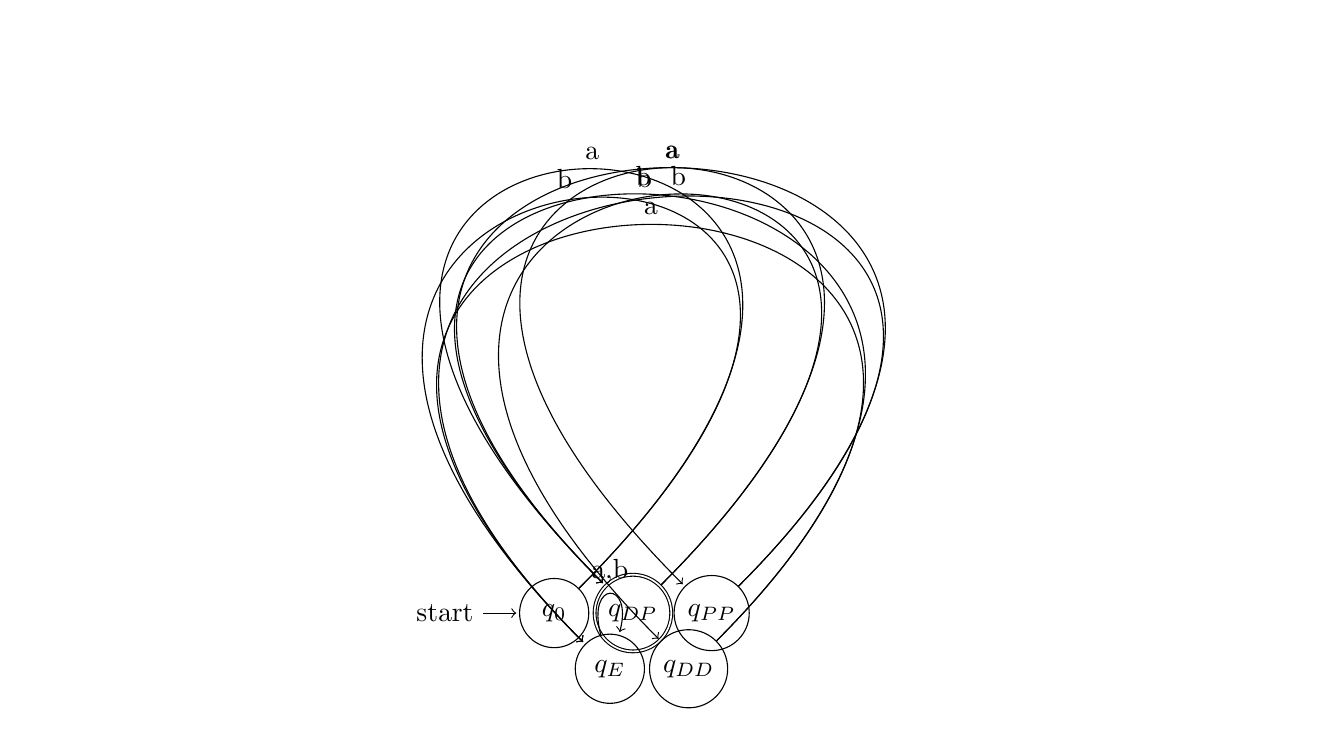
\begin{tikzpicture}[shorten >=1pt, distance = 10cm,on grid, auto]
  \node[state,initial] (q_0) {$q_0$};
  \node[state,accepting] (q_{DP}) [right of= q_0] {$q_{DP}$};
  \node[state] (q_E) [below right of= q_0] {$q_E$};
  \node[state] (q_{DD}) [below right of= q_{DP}] {$q_{DD}$};
  \node[state] (q_{PP}) [right of= q_{DP}] {$q_{PP}$};

  \path[->]
  (q_0) edge node [swap] {a} (q_{DP})
        edge node [swap] {b} (q_E)

  (q_{DP}) edge node [swap] {a} (q_{PP})
          edge node [swap] {b} (q_{DD})

  (q_{DD}) edge node [swap] {b} (q_{DP})
          edge node [swap] {a} (q_E)

  (q_{PP}) edge node [swap] {a} (q_{DP})
          edge node [swap] {b} (q_E)

  (q_E) edge [loop above] node {a,b} ();
\end{tikzpicture}

%Automa che termina per d con un numero pari di d

%Automa per disegnare aa^*cc^*d
\begin{tikzpicture}[shorten >= 1pt, distance = 10cm, on grid, auto]
  \node[state,initial] (q_0) {$q_0$};
  \node[state] (q_1) [right of = q_0] {$q_1$};
  \node[state] (q_E) [below right of= q_0] {$q_E$};
  \node[state] (q_2) [right of = q_1] {$q_2$};
  \node[state,accepting] (q_3) [right of = q_2] {$q_3$};

  \path[->]
  (q_0) edge node [swap] {a} (q_1)
        edge node [swap] {b,c,d} (q_E)

  (q_1) edge [loop above] node {a} ()
        edge node [swap] {c} (q_2)
        edge node [swap] {b,d} (q_E)

  (q_2) edge [loop above] node {c} ()
        edge node [swap] {d] (q_3)
        edge node [swap] {a,b} (q_E)
        (q_3) edge node [swap] {a,b,c,d} (q_E)
  (q_E) edge [loop above] node {a,b,c,d} ();
\end{tikzpicture}
\end{document}







































    1\4'
    

Esercizio:Gli studenti che non si iscrivono all'appello di Fondamenti non possono svolgere l'esame

Costanti:$Fondamenti$
Predicati:$Studente(x)$,$Iscrivere(x,y)$,$Svolgere(x,y)$,$Esame(y)$
Funzioni:
\begin{equation*}
\forall x (Studente(x) \land \neg Iscrivere(x,Fondamenti) \rightarrow
\exists y (Esame(y) \land \neg Svolgere(x,y)))
\end{equation*}

Esercizio:Tutti i professori fanno esami

Costanti: non presenti \newline
Predicati:$Professore(x)$,$Fare(x,y)$,$Esame(y)$ \newline
Funzioni: non presenti
\begin{equation*}
    \forall x (Professore(x) \rightarrow \exists y(Esame(y) \land Fare(x,y)))
\end{equation*}

Esercizio: Se uno studente non è iscritto via Sifa ad un appello non può fare l'esame

Costanti: non presenti \newline
Predicati:$Studente(x)$,$Iscritto(x,y)$,$Appello(y)$,$Esame(x)$ \newline
Funzioni: non presenti
\begin{equation*}
    \forall x (Studenti(x) \land \exists y(Appello(y) \land \neg Iscritto(x,y)) \rightarrow \neg Esame(x))
\end{equation*}

Esercizio: il voto di un esame universitario va da 0 a 30 e lode

Costanti:$0$ e $30L$ \newline
Predicati:$Esame(x)$,$>=(x,y)$,$<=(x,y)$ \newline
Funzioni:$voto(x)$
\begin{equation*}
    \forall x (Esame(x) \rightarrow voto(x) >= 0 \land voto(x) <= 30L)
\end{equation*}

Esercizio:Tutti i docenti sono sposati con una donna antipatica

Costanti: non presenti \newline
Predicati:$Docente(x)$,$Donna(y)$,$Sposati(x,y)$,$Antipatica(y)$ \newline
Funzioni: non presenti
\begin{equation*}
    \forall x (Docente(x) \rightarrow \exists y(Donna(y) \land Antipatica(y) \land Sposati(x,y)))
\end{equation*}

Esercizio:Marco ha un capo magnanimo

Costanti:$Marco$ \newline
Predicati:$Capo(x,y)$,$Magnanimo(x)$ \newline
Funzioni: non presenti \newline
\begin{equation*}
    Capo(x,Marco) \land Magnanimo(x)
\end{equation*}

Esercizio:L'everest è la montagna più alta al mondo

Costanti:$Everest$ \newline
Predicati:$Montagna(x)$,$<(x,y)$ \newline
Funzioni:$altezza(x)$
\begin{equation*}
    \forall x (Montagna(x) \rightarrow altezza(x) < altezza(Everest))
\end{equation*}

Esercizio:Se ogni amico di Mario è amico di Diego e Pietro non è amico di
          Mario, allora Pietro non è amico di Diego

Costanti:$Mario$,$Diego$,$Pietro$ \newline
Predicati:$Amico(x,y)$ \newline
Funzioni:non presenti
\begin{equation*}
    \forall x (((Amico(x,Mario) \rightarrow Amico(x,Diego)) \land \neg Amico(Pietro,Mario))
                \rightarrow \neg Amico(Pietro,Diego))
\end{equation*}

